% L14a student companion deck: updating the single index model and paper trading.
% The review (jump hidden Markov models and the sector factor model, with the carried-over
% sector factor example), the Alpaca company profile, the daily update of the single index
% model by exponentially weighted least squares, the preference weights with the updated
% estimates and their comparison with betting against beta, paper trading through an AI
% assistant and the MCP server, the order types and the life of an order, the three examples,
% the optional advanced material, and the summary.
%
% November 19, 2026: first build. The frame order mirrors the lecture notebook, and every
% sentence comes from it. The review copies the L13b review frame and the L13b sector factor
% definition frame. The paper trading figure is figs/Fig-L14a-PaperTrading-Schematic.pdf.
% The disclaimer is slide 2, by instructor preference.
% Notation follows the lecture: the EWLS decay phi = 2^(-1/63), the prior weight N_0 = 63,
% the updated estimates alpha_i(t) and beta_i(t), and the preference weight gamma_i(t).
\documentclass[aspectratio=169,11pt]{beamer}
\usepackage{vnslides}

\newcommand{\repo}{https://github.com/varnerlab/CHEME-5660-CourseRepository-Fall-2026/blob/main/lectures/week-14/L14a}

\title{\texorpdfstring{{\vnheavy L14a}}{L14a}: Updating the Single Index Model and Paper Trading}
\subtitle{CHEME 5660 Cornell University}
\author{Copyright Jeffrey Varner 2026. All Rights Reserved}

\begin{document}

\vntitlepage

\begin{frame}{Disclaimer and Risks}
  \vspace{0.6em}
  \textbf{\ink{Training only.}} This content is for training and informational
  purposes only. The teaching team does not make, give, or endorse any offer or
  solicitation to buy or sell securities or derivative products, or provide
  investment or trading advice or strategy.

  \vspace{1.1em}
  \textbf{\ink{Risk.}} Trading involves risk and is generally not recommended for
  those with limited resources, experience, or a low risk tolerance. Past
  performance does not guarantee future success.

  \vspace{1.1em}
  \textbf{\ink{Responsibility.}} You are responsible for your investment decisions
  based on your financial circumstances, objectives, risk tolerance, and
  liquidity needs.
\end{frame}

\begin{frame}{Objectives for Today}
  Previously, we held each stock's market sensitivity at its 2014 to 2024 estimate. How do
  we keep the estimate current as new trading days arrive, and how do we send orders for the
  stocks we pick?

  \vspace{0.5em}
  {\large\textbf{\ink{Today's concepts}}}
  \begin{itemize}\setlength{\itemsep}{0.4em}
    \item \hilite{Updating the single index model}: update each stock's baseline and market
      sensitivity with each new trading day by exponentially weighted least squares.
    \item \hilite{Updated preference weights}: pick a new $\gamma$ basket once a month and
      whenever the market turns, and compare its tilt with betting against beta.
    \item \hilite{Paper trading}: send orders for the $\gamma$ basket to a paper account, and
      follow each order until it fills or we cancel it.
  \end{itemize}
\end{frame}

\begin{frame}{What You Need to Know}
  \vspace{0.05em}
  {\large\textbf{\ink{Core concepts}}}
  \begin{itemize}\setlength{\itemsep}{0.05em}
    \item Exponentially weighted least squares updates each stock's single index estimates
      every trading day. Recent days count the most, because the weight of a day of data
      halves every 63 trading days.
    \item The preference weight uses the updated estimates and the market state $\xi_{t}$.
      When the market falls, it favors stocks with a low market sensitivity, the bet of
      betting against beta.
    \item A trading API lets a program check an account, read prices, and send orders. A
      paper account trades simulated money at real market prices.
  \end{itemize}

  \vspace{0.3em}
  {\large\textbf{\ink{For understanding}} \dimmed{(you won't reproduce these)}}
  \begin{itemize}\setlength{\itemsep}{0.2em}
    \item The derivation of the daily update from the weighted least-squares problem.
    \item The rules for picking the $\gamma$ basket: the sector quota, the floor on the market
      sensitivity, and the market-turn rule.
    \item How the MCP server turns a request in plain English into calls to Alpaca's API.
  \end{itemize}
\end{frame}

\begin{frame}{Lectures and Examples}
  \vspace{0.3em}
  {\normalsize\textbf{\ink{Lecture:}}\par\small
  \href{\repo/CHEME-5660-L14a-Lecture-UpdatingSIM-PaperTrading-Fall-2026.ipynb}{\dimmed{CHEME-5660-L14a-Lecture-UpdatingSIM-PaperTrading-Fall-2026.ipynb}}}

  \vspace{0.6em}
  {\normalsize\textbf{\ink{Examples:}}\par\small
  \href{\repo/CHEME-5660-L14a-Example-JumpHMM-SectorFactor-Fall-2026.ipynb}{\dimmed{CHEME-5660-L14a-Example-JumpHMM-SectorFactor-Fall-2026.ipynb}}\par
  \href{\repo/CHEME-5660-L14a-Example-Updating-SIM-Gamma-Fall-2026.ipynb}{\dimmed{CHEME-5660-L14a-Example-Updating-SIM-Gamma-Fall-2026.ipynb}}\par
  \href{\repo/alpaca-mcp/README.md}{\dimmed{alpaca-mcp/README.md}}}

  \vspace{0.6em}
  Optional advanced notebooks are listed on the Optional Advanced Material frame.
\end{frame}

% ========== Review: jump hidden Markov models and the sector factor model
\begin{frame}{Review: Jump Hidden Markov Models}
  The model bins the daily growth rate into states of equal probability and estimates the
  transition matrix by counting moves between states. Each day, the chain takes one step,
  and the model draws the growth rate from the new state:
  \begin{center}
    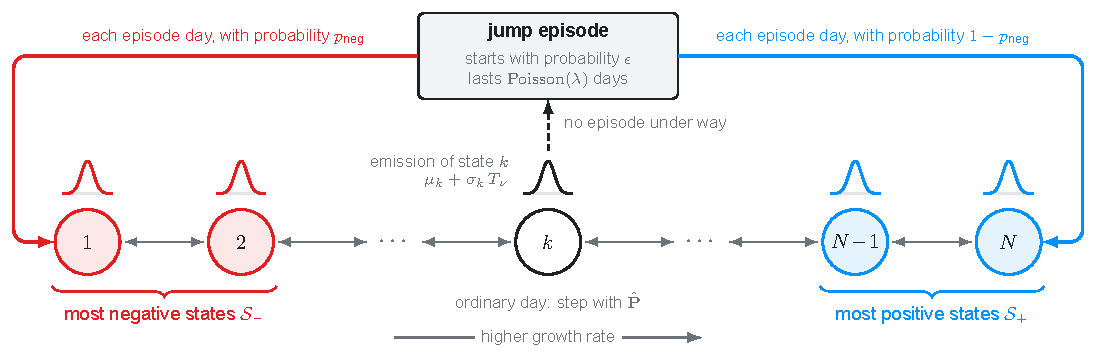
\includegraphics[width=\textwidth,height=0.42\textheight,keepaspectratio]{../figs/Fig-L13b-JumpHMM-Schematic.pdf}
  \end{center}
  Jump episodes start at random and last several days. On each episode day, the state comes from
  the most negative or the most positive states. These runs of large moves add the volatility
  clustering that the chain alone misses.
\end{frame}

\begin{frame}{Review: The Sector Factor Model}
  Then we extended the jump hidden Markov model to many stocks that move together. A
  \hilite{sector factor model} adds one factor for each sector of the
  \href{https://www.msci.com/our-solutions/indexes/gics}{Global Industry Classification Standard (GICS)}.
  Each sector factor describes how the single index residuals of the stocks in its sector move
  together:
  \begin{equation*}
    g_{i}(t)=\underbrace{\alpha_{i}}_{\textstyle\text{baseline}}+\underbrace{\beta_{i}\,g_{m}(t)}_{\textstyle\text{market}}+\overbrace{\underbrace{\delta_{i}\,f_{s}(t)}_{\textstyle\text{sector}}+\underbrace{u_{i}(t)}_{\textstyle\text{stock-specific}}}^{\textstyle\text{single index residual }\varepsilon_{i}(t)}
  \end{equation*}
  Here $g_m(t)$ is the growth rate of \texttt{SPY}, $f_s(t)$ is the growth rate of sector $s$
  (with the market part removed), and $u_i(t)$ is the growth rate that neither the market nor the
  sector explains. The market sensitivity $\beta_{i}$ and the sector loading $\delta_{i}$ set how much
  stock $i$ moves with the market and with its sector.

  \vspace{0.4em}
  We built the many-stock model from single-asset jump hidden Markov models: one for the market,
  one for each sector, and one for each stock.
\end{frame}

\begin{frame}{Example: A Synthetic Market of Many Stocks}
  \vspace{0.3em}
  {\normalsize\textbf{\ink{Example:}}\par\small
  \href{\repo/CHEME-5660-L14a-Example-JumpHMM-SectorFactor-Fall-2026.ipynb}{\dimmed{CHEME-5660-L14a-Example-JumpHMM-SectorFactor-Fall-2026.ipynb}}}

  \vspace{0.8em}
  In this example, we use the sector factor model to build a universe of \texttt{SPY} and 375
  stocks from all 11 sectors. We compare the correlations, volatilities, and market sensitivities
  of a synthetic path with the real data, and the stylized facts of one synthetic stock, with and
  without jumps, with its real growth rates. Then we save the fitted model.

  \vspace{0.8em}
  \textbf{\ink{Today:}} we update the single index model with each new trading day, pick stocks
  with the updated preference weights, and send orders for those stocks to a paper account.
\end{frame}

% ========== Company profile: Alpaca
\begin{frame}{Company Profile: Alpaca}
  \href{https://alpaca.markets/about}{\hilite{Alpaca}}: a brokerage built for programs that
  trade, founded in 2015 by Yoshi Yokokawa and Hitoshi Harada. Its customers send orders through
  an application programming interface (API).
  \begin{itemize}\setlength{\itemsep}{0.25em}
    \item \hilite{Trading for programs}: the Trading API lets a program check an account, read
      prices, and send orders. Every user gets a free paper trading account.
    \item \hilite{Brokerage for other apps}: in January 2026, Alpaca raised 150 million USD and
      reported over 9 million brokerage accounts in more than 40 countries.
    \item \hilite{AI assistants that trade}: Alpaca maintains an official Model Context Protocol
      (MCP) server, and raised 135 million USD in July 2026 for ``agent-first'' brokerage.
  \end{itemize}
  \textbf{\ink{Connection:}} we'll send orders for the $\gamma$ basket to an Alpaca paper account
  through our own MCP server.
  \slidenote{Video:}{\href{https://www.youtube.com/embed/KiWT1qq59Gc}{Backend Operations for a Trade (2023)}.}
\end{frame}

% ========== Updating the single index model
\begin{frame}{Updating the Single Index Model}
  A stock's market sensitivity changes over time. We update the estimates with each new trading
  day, giving recent days the most weight.

  \vspace{0.3em}
  \textbf{\ink{Exponentially weighted least squares (EWLS):}} on trading day $t$, the updated
  baseline $\alpha_{i}(t)$ and market sensitivity $\beta_{i}(t)$ of stock $i$ solve:
  {\small\begin{equation*}
    \left(\alpha_{i}(t),\beta_{i}(t)\right)=\arg\min_{a,\,b}\Biggl[\underbrace{\sum_{k=t_{0}+1}^{t}\phi^{\,t-k}\left(g_{i}(k)-a-b\,g_{m}(k)\right)^{2}}_{\textstyle\text{weighted data}}+\underbrace{\phi^{\,t-t_{0}}N_{0}\,\mathbb{E}_{0}\left[\left(g_{i}-a-b\,g_{m}\right)^{2}\right]}_{\textstyle\text{prior}}\Biggr]
  \end{equation*}}
  where $g_{i}(k)$ and $g_{m}(k)$ are the daily growth rates of stock $i$ and \texttt{SPY} on day $k$
  (1/yr), $a$ and $b$ are a candidate baseline and market sensitivity, and $t_{0}$ is the last day of
  the fitting period. The prior weight $N_{0}=63$ counts the 2014 to 2024 fit as 63 days of data, and
  $\mathbb{E}_{0}$ is the expected value under that fit.
\end{frame}

\begin{frame}{The Parts of the Update}
  Each part of the problem has a job:
  \begin{itemize}\setlength{\itemsep}{0.45em}
    \item \hilite{Weighted data}: each day, the weight of every earlier day shrinks by
      $\phi=2^{-1/63}$, which halves it every 63 trading days. The new day enters with weight one.
    \item \hilite{Prior}: the prior term is the expected squared residual under the 2014 to 2024 fit.
      On the first day, the prior alone gives the 2014 to 2024 estimates, and after a year of
      trading it carries little weight.
    \item \hilite{No look-ahead}: the estimates on day $t$ use the growth rates through day $t$.
      The trading method decides after the close of day $t$ and trades at the next open.
  \end{itemize}
  \vspace{0.3em}
  We use the EWLS recursion, which updates the estimates from a few running sums instead of
  storing every past day.
  \slidenote{Derivation:}{\href{\repo/advanced/ewls/CHEME-5660-L14a-Derivation-EWLS-Update-Fall-2026.ipynb}{The EWLS recursion (advanced notebook)}.}
\end{frame}

\begin{frame}{Preference Weights with Updated Estimates}
  Previously, we computed the preference weight $\gamma_{i}(t)$ from the single index estimates,
  the recent market growth rate $\tilde{g}_{M,t}$, and the market state $\xi_{t}$. The trading
  method of \href{https://arxiv.org/abs/2611.03022}{Varner (2026)} uses it with the updated
  estimates:
  \begin{equation*}
    \boxed{\gamma_{i}(t)=\tanh\left(h\,\frac{\alpha_{i}(t)+\beta_{i}(t)\,\tilde{g}_{M,t}}{\max\left(|\beta_{i}(t)|,\,\beta_{\text{floor}}\right)^{\xi_{t}}}\right)}
  \end{equation*}
  where the horizon $h=1$ year makes the argument of the $\tanh$ dimensionless, and the floor is
  $\beta_{\text{floor}}=0.1$. The market state $\xi_{t}$ is positive when the market has recently
  been falling, and negative when it has been rising.
  \begin{itemize}\setlength{\itemsep}{0.1em}
    \item \hilite{Floor}: the denominator uses $|\beta_{i}(t)|$ with a floor, which keeps the
      preference weight defined for every stock.
    \item \hilite{Picks at market turns}: the \hilite{$\gamma$ basket} holds the three stocks with
      the highest preference weights in each sector. The method picks a new basket every 21 trading
      days, and whenever $\xi_{t}$ moves to the other side of zero.
  \end{itemize}
\end{frame}

\begin{frame}{The Market Hedge}
  With a \hilite{market hedge}, the trading method limits the market sensitivity of the whole
  portfolio on each day it sets its holdings:
  \begin{equation*}
    \boxed{\beta_{P}(t)=\sum_{i}w_{i}(t)\,\beta_{i}(t)\leq\max\left(1-\xi_{t},\,-0.5\right)}
  \end{equation*}
  where $w_{i}(t)$ is the fraction of the portfolio's value in holding $i$, negative for a short.
  \begin{itemize}\setlength{\itemsep}{0.2em}
    \item \hilite{The limit}: one in a flat market ($\xi_{t}=0$) and zero at $\xi_{t}=1$. Because
      $|\xi_{t}|\leq 1$ on 99\% of training days, only a steep fall takes the limit below zero.
    \item \hilite{Meeting the limit}: the method can shift value toward the basket's stocks with a
      low market sensitivity, hold cash, which has a market sensitivity of zero, or buy up to five
      stocks whose market sensitivity is zero or negative.
    \item \hilite{Selling \texttt{SPY} short}: below zero, the method also sells \texttt{SPY} short.
      A limit of $-0.2$ gives a short worth 20\% of the portfolio's value.
  \end{itemize}
\end{frame}

\begin{frame}{The Trading Method and Betting Against Beta}
  \vspace{0.05em}
  {\large\textbf{\ink{How does the trading method compare with betting against beta?}}}

  \vspace{0.2em}
  Previously, we met \href{https://www.aqr.com/Our-Firm/About-Us}{AQR Capital Management}, where Andrea
  Frazzini and Lasse H. Pedersen proposed the
  \href{https://www.aqr.com/Insights/Research/Journal-Article/Betting-Against-Beta}{betting-against-beta portfolio}
  in 2014. Their portfolio always buys stocks with a low market sensitivity and sells stocks with
  a high one, in amounts that make its market sensitivity zero. The trading method makes the same
  bet only when the market falls:

  \vspace{0.2em}
  \begin{itemize}\setlength{\itemsep}{0.2em}
    \item \hilite{Signal}: when the market falls ($\xi_{t}>0$), the preference weight favors stocks
      that move less with the market. When the market rises ($\xi_{t}<0$), the tilt reverses.
    \item \hilite{Long-only basket}: the $\gamma$ basket keeps the three stocks with the highest
      preference weights in each sector. A low-weight stock is left out, not sold short.
    \item \hilite{Market hedge}: with the hedge on, the limit on $\beta_{P}(t)$ drops to zero, the
      market sensitivity of betting against beta, at $\xi_{t}=1$. After a steeper fall, the method
      sells \texttt{SPY} short, whereas betting against beta sells stocks with a high market
      sensitivity.
  \end{itemize}
\end{frame}

\begin{frame}{Example: Updating the Single Index Model}
  \vspace{0.3em}
  {\normalsize\textbf{\ink{Example:}}\par\small
  \href{\repo/CHEME-5660-L14a-Example-Updating-SIM-Gamma-Fall-2026.ipynb}{\dimmed{CHEME-5660-L14a-Example-Updating-SIM-Gamma-Fall-2026.ipynb}}}

  \vspace{0.8em}
  In this example, we update the single index model of every stock with each trading day of 2025
  and 2026, starting from the 2014 to 2024 fit. We pick the $\gamma$ basket once a month and
  whenever the market turns, and compare it with the basket that the fixed estimates pick.

  \vspace{0.8em}
  The example ends with the $\gamma$ basket of the last pick day in our data. Next, we send orders
  for the stocks of a basket to a paper trading account.
\end{frame}

% ========== Paper trading with Alpaca
\begin{frame}{Paper Trading with Alpaca}
  In a trading app, we send an order by tapping a button. A trading method decides its trades in
  a program, and the program sends its orders through Alpaca's API.

  \vspace{0.6em}
  \textbf{\ink{Definition:}} a \hilite{paper account} trades simulated money at real market
  prices. Alpaca fills each paper order against the latest quotes, and the order never reaches an
  exchange. A live account sends the same orders to the market with real money.

  \vspace{0.6em}
  A paper fill can differ from a live fill of the same order:
  \begin{itemize}\setlength{\itemsep}{0.25em}
    \item \hilite{Not simulated}: how our order moves the price, the order's place in line behind
      other orders, regulatory fees, and dividends.
    \item \hilite{Quotes}: the free quotes come from one exchange, IEX, and can show a wider
      bid-ask spread than the national best bid and offer.
  \end{itemize}
\end{frame}

\begin{frame}{Trading Through an AI Assistant}
  An \hilite{MCP server} gives an AI assistant one tool for each request to Alpaca:
  \begin{center}
    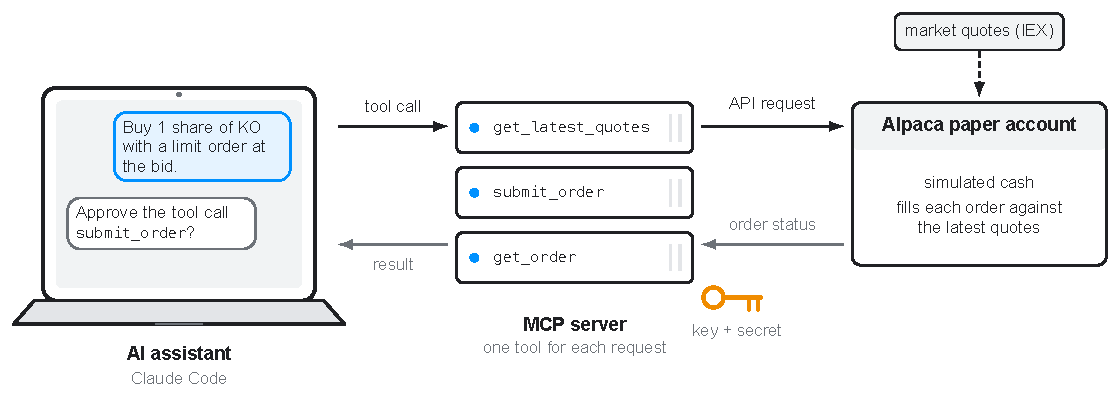
\includegraphics[width=\textwidth,height=0.66\textheight,keepaspectratio]{../figs/Fig-L14a-PaperTrading-Schematic.pdf}
  \end{center}
  The server holds the account's key and secret, and the assistant never sees them.
\end{frame}

\begin{frame}{Orders and Their Status}
  A \hilite{market order} fills right away at the best available price, but we do not know that
  price in advance. A \hilite{limit order} sets the worst price we accept, but it may not fill.

  \vspace{0.3em}
  Each order also has a \hilite{time in force}. A \texttt{day} order is canceled at the close if it
  has not filled, and a \texttt{gtc} order stays open until it fills or we cancel it:
  \begin{itemize}\setlength{\itemsep}{0.25em}
    \item \hilite{Open}: an order is \texttt{new} once Alpaca accepts it, and
      \texttt{partially\_filled} once some of its shares trade.
    \item \hilite{Done}: an order is \texttt{filled} when all of its shares trade, and
      \texttt{canceled} when we cancel it or a \texttt{day} order reaches the close.
    \item \hilite{Rejected}: an order is \texttt{rejected} when it fails a check before it can
      trade.
  \end{itemize}
  An unfilled limit order leaves the method holding fewer shares than it planned.
\end{frame}

\begin{frame}{Example: Paper Trade the $\gamma$ Basket}
  \vspace{0.3em}
  {\normalsize\textbf{\ink{Example:}}\par\small
  \href{\repo/alpaca-mcp/README.md}{\dimmed{alpaca-mcp/README.md}}}

  \vspace{0.8em}
  In this example, we connect Claude Code to an Alpaca paper account through an MCP server. We
  check the account and the quotes of the $\gamma$ basket, place limit orders for its stocks, and
  follow each order until it fills or we cancel it.
\end{frame}

% ========== Optional advanced material
\begin{frame}{Optional Advanced Material}
  \vspace{0.2em}
  {\normalsize\textbf{\ink{The daily update of the single index model:}} \dimmed{advanced/ewls/}\par
  \href{\repo/advanced/ewls/CHEME-5660-L14a-Derivation-EWLS-Update-Fall-2026.ipynb}{\dimmed{CHEME-5660-L14a-Derivation-EWLS-Update-Fall-2026.ipynb}}}

  \vspace{0.3em}
  We derive the running sums that the exponentially weighted least squares update carries from
  one day to the next. We solve them for the updated estimates and the residual standard deviation,
  and show how the 2014 to 2024 fit seeds the sums.
\end{frame}

\begin{frame}{Summary}
  \vspace{0.3em}
  We updated the single index model of every stock with each trading day, picked the $\gamma$
  basket from the updated preference weights, and sent orders for a basket to a paper account.

  \vspace{0.4em}
  {\large\textbf{\ink{Key takeaways}}}
  \begin{itemize}\setlength{\itemsep}{0.4em}
    \item \hilite{Updating the single index model}: EWLS updates each stock's baseline and market
      sensitivity with every trading day. Over 2025 and 2026, the market sensitivity of most stocks
      fell below their fixed estimates.
    \item \hilite{Updated preference weights}: when the market fell, the $\gamma$ basket favored
      stocks with a low market sensitivity, as betting against beta does.
    \item \hilite{Paper trading}: we sent limit orders for the $\gamma$ basket to a paper account.
      Because a limit order may not fill, we followed each order until it filled or we canceled it.
  \end{itemize}
  \vspace{0.3em}
  The $\gamma$ basket says which stocks to consider. Deciding how many shares of each stock to buy,
  and when to trade, is the rest of the trading method.
\end{frame}

\end{document}
